\begin{figure}[htbp]
\centering
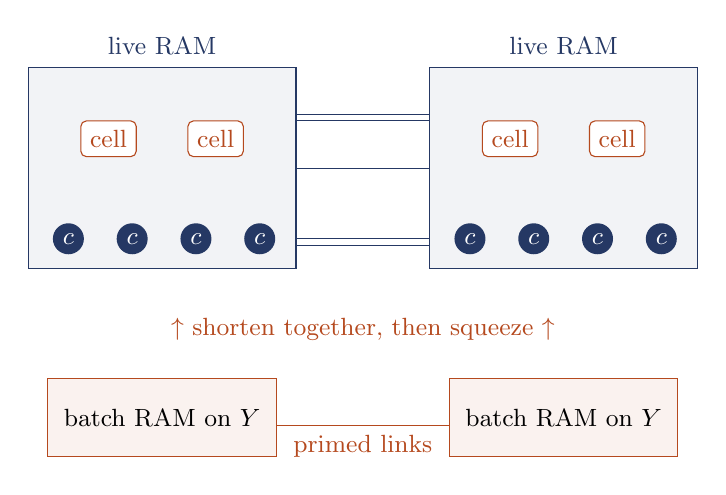
\begin{tikzpicture}[x=1cm,y=1cm,font=\small]
  \definecolor{live}{RGB}{37,56,100}
  \definecolor{primed}{RGB}{181,73,30}
  \foreach \offset in {0,5.1} {
    \begin{scope}[xshift=\offset cm]
      \draw[live,fill=live!6] (0,0) rectangle (3.4,2.55);
      \node[live,above] at (1.7,2.6) {live RAM};
      \foreach \x in {1.02,2.38}
        \node[draw=primed,text=primed,fill=white,rounded corners=2pt]
          at (\x,1.65) {cell};
      \foreach \x in {0.51,1.32,2.13,2.94}
        \node[circle,fill=live,text=white,inner sep=2pt] at (\x,.38) {$c$};
      \draw[primed,fill=primed!7] (.25,-2.38) rectangle (3.15,-1.40);
      \node at (1.7,-1.89) {batch RAM on $Y$};
    \end{scope}
  }
  \foreach \y in {.30,.38,1.275,1.88,1.96}
    \draw[live] (3.4,\y) -- (5.1,\y);
  \node[primed] at (4.25,-.77) {$\uparrow$ shorten together, then squeeze $\uparrow$};
  \draw[primed] (3.15,-1.99) -- (5.35,-1.99)
    node[midway,below] {primed links};
\end{tikzpicture}
\caption{What gets replayed (two of many teams). A batch RAM sees even the code for the live
simulation but uses it only as slot addresses, not as code. Pieces from many primed teams can end
up inside the same cell, and the cells migrate to live teams as determined by a public ledger.}
\label{fig:replay}
\end{figure}
